\begin{frame}{PERMANOVAs - all kids}
    \begin{columns}[c] % The "c" option specifies centered vertical alignment while the "t" option is used for top vertical alignment

        \column{.6\textwidth} % Right column and width
    
        \begin{figure}
        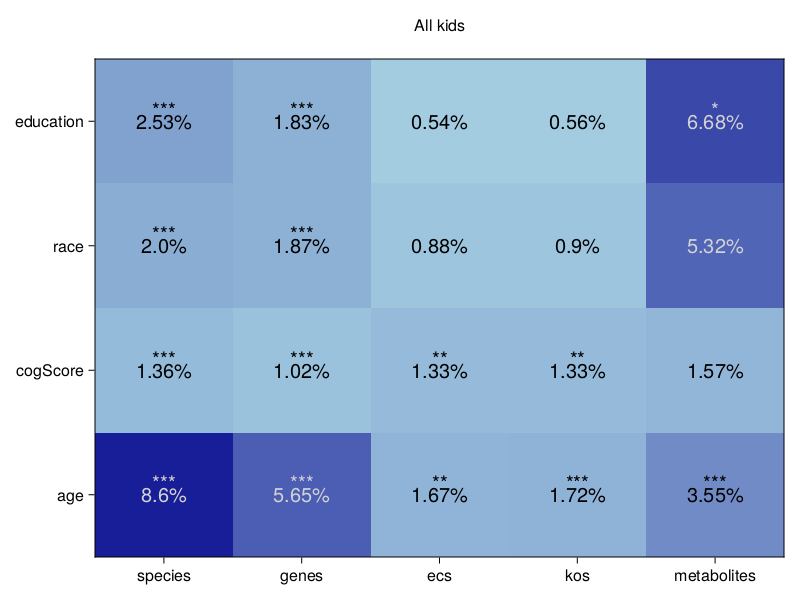
\includegraphics[width=1\linewidth]{../figures/kids_all_permanovas.png}
        \end{figure}

        \column{.4\textwidth} % Right column and width
    
        \textbf{Details}
        \begin{itemize}
            \item Single sample (first) per kid
            \item Univariate permanova
            \item For KOs / ECs, UNGROUPED features were excluded, UNMAPPED were included
        \end{itemize}

    \end{columns}

\end{frame} 

\begin{frame}{PERMANOVAs - kids under 6 months old}
    \begin{columns}[c] % The "c" option specifies centered vertical alignment while the "t" option is used for top vertical alignment

        \column{.6\textwidth} % Right column and width
    
        \begin{figure}
        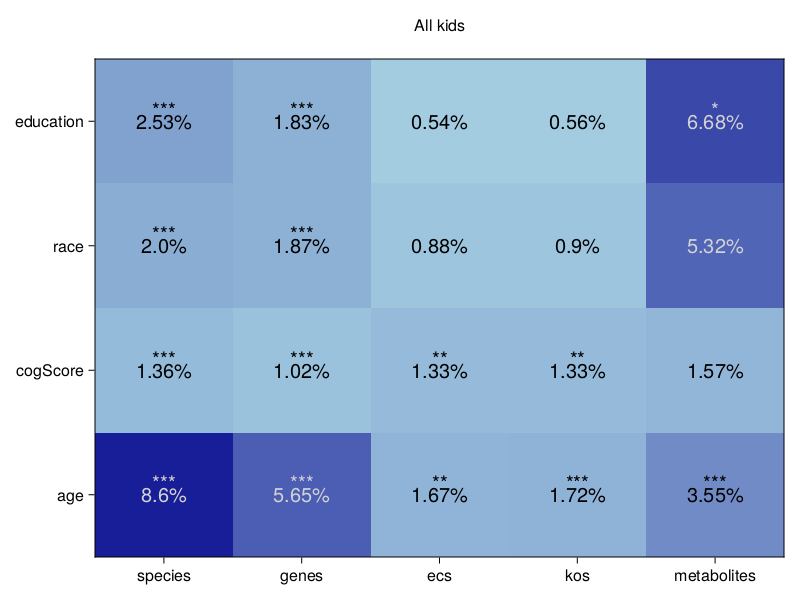
\includegraphics[width=1\linewidth]{../figures/kids_all_permanovas.png}
        \end{figure}

        \column{.4\textwidth} % Right column and width
    
        \textbf{Details}
        \begin{itemize}
            \item Single sample per kid
            \item Univariate permanova
            \item For KOs / ECs, UNGROUPED features were excluded, UNMAPPED were included
        \end{itemize}

    \end{columns}

\end{frame}

\begin{frame}{PERMANOVAs - kids over 1 year old}
    \begin{columns}[c] % The "c" option specifies centered vertical alignment while the "t" option is used for top vertical alignment

        \column{.6\textwidth} % Right column and width
    
        \begin{figure}
        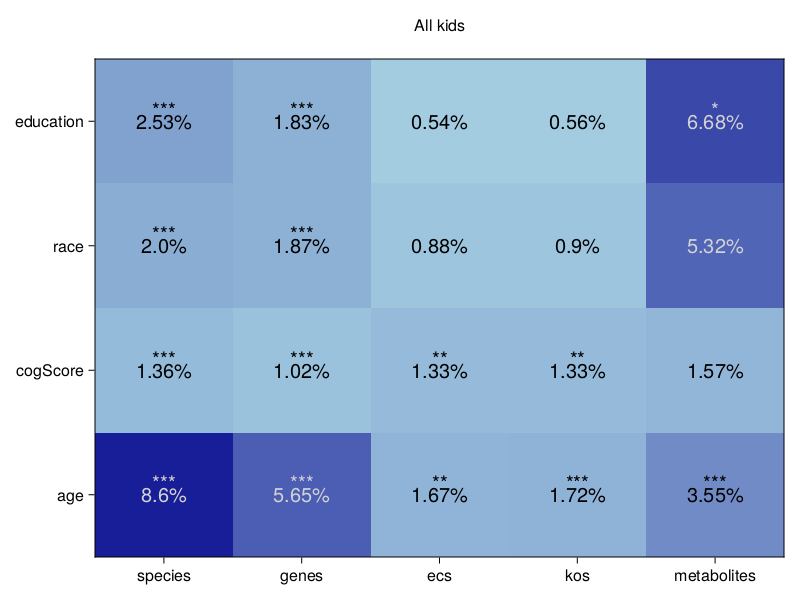
\includegraphics[width=1\linewidth]{../figures/kids_all_permanovas.png}
        \end{figure}

        \column{.4\textwidth} % Right column and width
    
        \textbf{Details}
        \begin{itemize}
            \item Single sample per kid
            \item Univariate permanova
            \item For KOs / ECs, UNGROUPED features were excluded, UNMAPPED were included
            \item Metabolites not included because there are only a few samples over 1 year
        \end{itemize}

    \end{columns}

\end{frame}


\begin{frame}{Linear models - taxa}
    \begin{columns}[c] % The "c" option specifies centered vertical alignment while the "t" option is used for top vertical alignment

        \column{.6\textwidth} % Right column and width
    
        \begin{figure}
        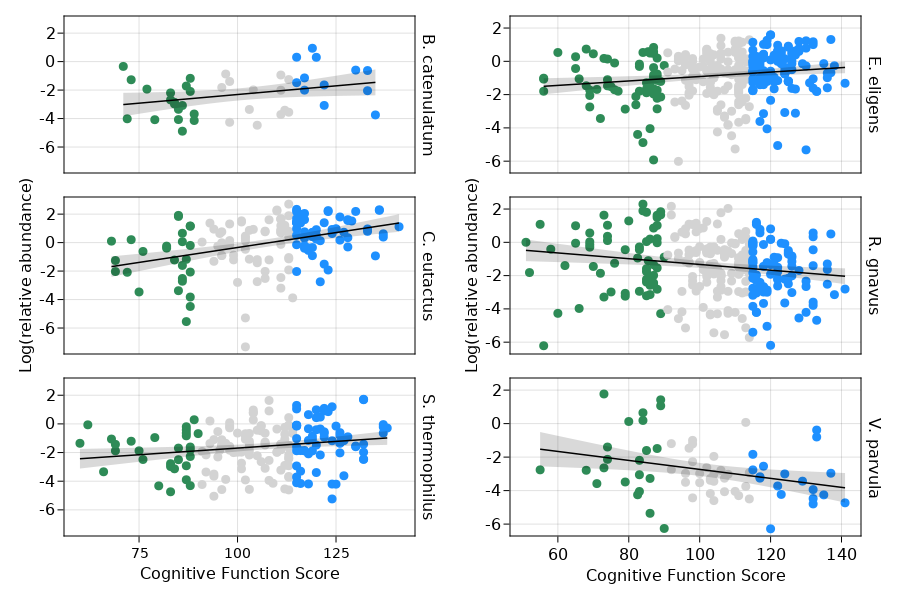
\includegraphics[width=1\linewidth]{../figures/lms-split-2.png}
        \end{figure}

        \column{.4\textwidth} % Right column and width
    
        \textbf{Details}
        \begin{itemize}
            \item Kids $> 18$ months old, species $> 10\%$ prevalence
            \item GLM: $bug \sim cogScore + age$
            \item There were ~15 bugs significant after FDR correction
        \end{itemize}

    \end{columns}

\end{frame}

\begin{frame}{Linear models - taxa}
    \begin{columns}[c] % The "c" option specifies centered vertical alignment while the "t" option is used for top vertical alignment

        \column{.6\textwidth} % Right column and width
    
        \begin{figure}
        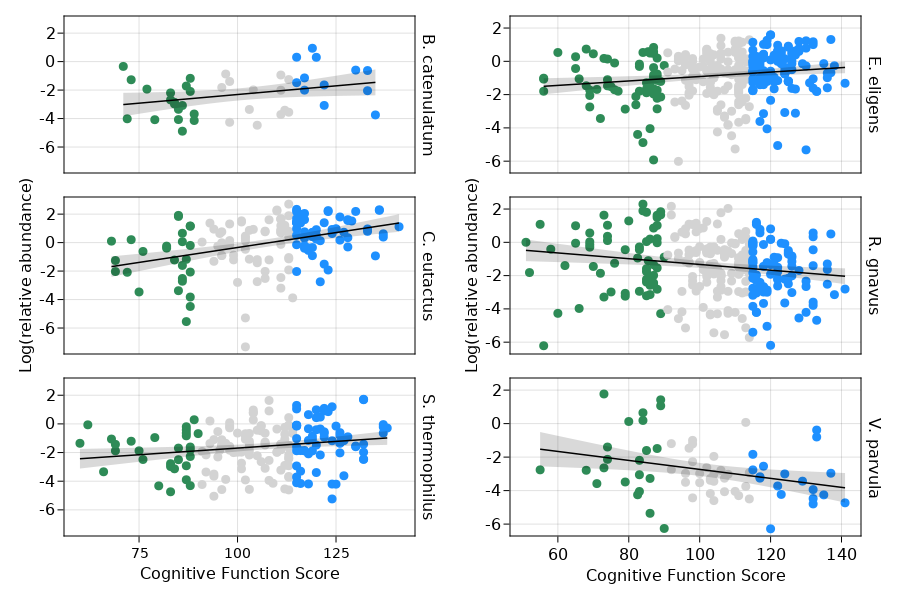
\includegraphics[width=1\linewidth]{../figures/lms-split-2.png}
        \end{figure}

        \column{.4\textwidth} % Right column and width
    
        \textbf{Details}
        \begin{itemize}
            \item Kids $> 18$ months old, species $> 10\%$ prevalence
            \item GLM: $bug \sim cogScore + age$
            \item There were ~15 bugs significant after FDR correction
        \end{itemize}

    \end{columns}

\end{frame}